 \chapter{Background}
 \section{Introduction}

 In this chapter, we present the background necessary to appreciate our proposed method based on image texture and r Random forest. We show a generic overview of various min concepts, while the more specific details of different techniques in relevant chapters. 
 
 Facial expression recognition field has started being discussed during the end of the last century \citep{essa1995facial}. Since then, many researchers have proposed method to improve machine ability to recognise human facial expressions.   

 
\section{Active shape model And  Active appearance model}
An active appearance model (AAM) \citep{edwards1998interpreting, cootes1998activeApearance,cootes2001active} is a computer vision algorithm depends on  statistical finding the values are fit with a grey image's texture values, and make a statistical linking with an active shape model \citep{cootes1992active,cootes1992training,cootes1995active}.
ASM was first proposed by \citet{cootes1992active} based on models created from sets of training examples called Point Distribution Models (PDM), represent objects as sets of labelled points called landmark points. Figure \ref{fig:PDM} illustrates a PDM as an example of face points landmarking. AAM was first proposed by \citet{edwards1998interpreting} for face analysis. Since that the method has  been common used in computer vision applications such as matching and tracking faces and for medical image analysis. 

The training example set are labelled manually, each shape is represented as shown in equation \ref{equ:points}. The first step is computing the mean points for all the training set to find the mean shape $\boldsymbol{\bar{x}}$. 
%%%%%%%%%%%%%%%%%%%%%%%%%%%%%%%%%%%%%%%%%%%%%%%%%%%%%%%%%%%%%%%%%
\begin{equation}
\boldsymbol{x} = (x_0, y_0 , x_1, y_1,  ..., x_k, y_k, ..., x_{n-1}, y_{n-1})^T
    \label{equ:points}
\end{equation}
%%%%%%%%%%%%%%%%%%%%%%%%%%%%%%%%%%%%%%%%%%%%%%%%%%%%%%%%%%%%%%%%%
where $ (x_k, y_k$)is the position point $k$ 

AAM's idea is to combine a model of face shape variation with a model of the appearance variations of a shape-normalised face.
 In order to create new shapes from the mean shape $\boldsymbol{\bar{x}}$, ASM variate modes. To achieve that, Principal components analysis (PCA) is applied on all training data to calculate eigenvectors of the covariance matrix. To Generate a new shape the following equation is used:
%%%%%%%%%%%%%%%%%%%%%%%%%%%%%%%%%%%%%%%%%%%%%%%%%%%%%%%%%%%%%%%%%
\begin{equation}
\boldsymbol{x} \approx \boldsymbol{\bar{x}} + \boldsymbol{P}_s \boldsymbol{b}_s
    \label{equ:NewShapes}
\end{equation}
%%%%%%%%%%%%%%%%%%%%%%%%%%%%%%%%%%%%%%%%%%%%%%%%%%%%%%%%%%%%%%%%%
where $\boldsymbol{\bar{x}}$ the mean shape, $\boldsymbol{P}= (\boldsymbol{P}_1 \mid \boldsymbol{P}_2\mid...\mid \boldsymbol{P}_t)$  contains t eigenvectors of the covariance matrix and $\boldsymbol{b}$ is a t dimensional vector given by

%%%%%%%%%%%%%%%%%%%%%%%%%%%%%%%%%%%%%%%%%%%%%%%%%%%%%%%%%%%%%%%%
\begin{equation}
\boldsymbol{b} = \boldsymbol{P}^T (\boldsymbol{x-\bar{x}})
    \label{equ:points}
\end{equation}
%%%%%%%%%%%%%%%%%%%%%%%%%%%%%%%%%%%%%%%%%%%%%%%%%%%%%%%%%%%%%%%%%
 
 All image shapes are normalised to the mean shape, then each image is warped to its control points the same pose (translation, scale and rotation) values used in shapes normalisation, so we can sample the grey level information $\boldsymbol{g}$ from shape-normalised face patch. By applying PCA to this data we obtain this model:
 

%%%%%%%%%%%%%%%%%%%%%%%%%%%%%%%%%%%%%%%%%%%%%%%%%%%%%%%%%%%%%%%%
\begin{equation}
\boldsymbol{g} \approx \boldsymbol{\bar{g}} + \boldsymbol{P}_g \boldsymbol{b}_g
    \label{equ:NewGreys}
\end{equation}
%%%%%%%%%%%%%%%%%%%%%%%%%%%%%%%%%%%%%%%%%%%%%%%%%%%%%%%%%%%%%%%%%

A further PCA is applied to correlated shape and grey-level variations, to obtain:

\begin{equation}
\boldsymbol{x} \approx \boldsymbol{\bar{x}} + \boldsymbol{Q}_s \boldsymbol{c}
    \label{equ:ModelNewShapes}
\end{equation}

\begin{equation}
\boldsymbol{g} \approx \boldsymbol{\bar{g}} + \boldsymbol{Q}_g \boldsymbol{c}
    \label{equ:ModelNewShapes}
\end{equation}

By varying the elements of $\boldsymbol{c}$ in equation \ref{equ:ModelNewShapes} and \ref{equ:NewGreys}, new shapes and images will be generated. So $c_i$ is the variance of the $i_{th}$  parameter given by  $ \lambda_i$. To generate similar shapes to the original training data, limits of $\pm3 \sqrt[]{\lambda_i}$ have been applied to the parameter $b_i$. 

Now if we given a new image $\boldsymbol{I}$ and we want to find the shape points are fit to the image we need to vary $\boldsymbol{c}$ to generate new images, the finding the most slimier generated image for the appearance model to $\boldsymbol{I}$.  This is an optimisation problem to find the best $\boldsymbol{c}$ efficiently, which will generate shape landmarks which describe the face parts. 




%%%%%%%%%%%%%%%%%%%%%%%%%%%%%%%%%%%%%%%%%%%%%%%%%%%%%%%%%%%%%%%%%
\begin{figure}[H]
\centering
  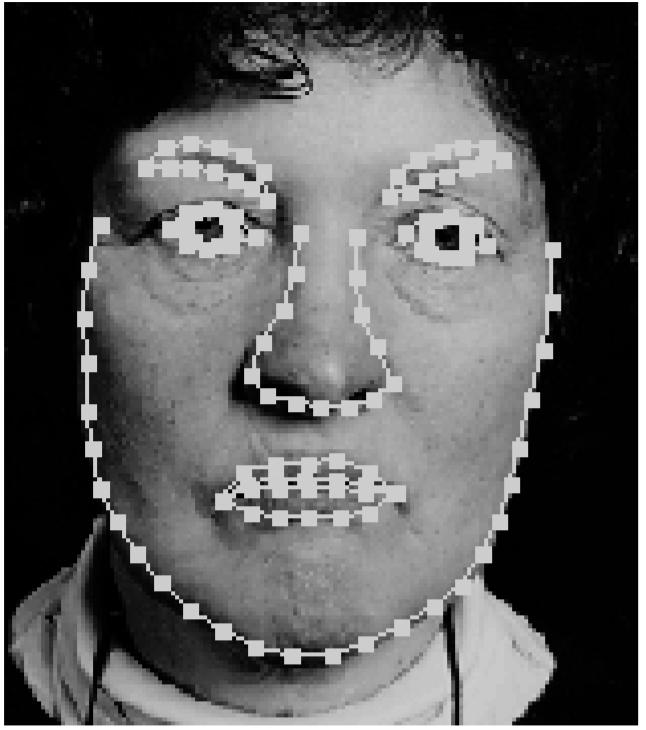
\includegraphics[width=0.3\textwidth]{Chapter2/Figs/FacePoints.png}
  \textbf{
    \caption{Point Distribution Model}
    \label{fig:PDM}}
\end{figure}
%%%%%%%%%%%%%%%%%%%%%%%%%%%%%%%%%%%%%%%%%%%%%%%%%%%%%%%%%%%%%%%%%



Since \citet{edwards1998interpreting} many researches have used AAM in many applications  recognise facial expression in f videos \cite{sung2006real, martin2008real} and photos \cite{kanade2000comprehensive, van2005model,wu2013facial} . Facial expressions recognition one the most topics has been discussed during the last three decades. Researches applied AAM to extract facial features face point to be classified using various classifiers. One of the ways that AAM has been used to in facial recognition system is to detect action unit described the Facial Action Coding System (FACS) \cite{ekman1978facial} which based on minimal muscular movements  and which individually or in combinations  represent all facial expressions \citep{cohn1998feature, van2005model,lucey2010extended} By finding  the action units exist in a face , and by use one or a group of them together, facial expression can be recognised. For instant, AU1 is Inner Brow Raiser, AU2 is Outer Brow Raiser, AU15 Lip Corner Depressor and AU28 Lip Suck. To determine Anger expression for example AU23 and AU24 must be present in the AU combination, where AU1+4+15 or 11 must be present for sadness \cite{lucey2010extended}. 
To classify the extracted features to find the AUs trained classifers has been used like neural networks trained with back propagation \citet{van2005model} on Cohn-Kanade AU-Coded (CK+) Facial Expression Database \citet{kanade2000comprehensive}, or Support Vector Machine (SVM) in \citet{lucey2010extended} with (CK+) database as well.     

On the other hand AAM was used for detect the facial expressions directly rather than AUs detection. The AAM features have classified with several classifiers such as simple Euclidean-distance classification scheme \cite{ratliff2008emotion},  K-means classification \cite{martins2008facial} or SVM \citet{pu2015facial}.






\section{Image texture based methods}
Image texture based or appearance-based methods have been widely used in computer vision applications face recognition and facial expressions recognition. The idea of image texture methods is using the image pixel values such as RGB, grey scale changes or illumination. Many methods have been proposed to describe the image  and extract the image features such as Locally Binary Patterns(LBP), Histogram of oriented gradients (HOG) scale-invariant feature transform (SIFT) and speeded up robust features (SURF).






%__________________________________________________________HOG__________________________________________________________________
%__________________________________________________________HOG__________________________________________________________________
%__________________________________________________________HOG__________________________________________________________________

\subsection{Local histogram of oriented gradients (HOG)}

Local histogram of oriented gradients (HOG) is a method proposed by Dalal et al.\citep{dalal2005histograms}. This method aims to describe an image with a set of local histograms. These histograms count occurrences of gradient orientation in a local part of the image. HOG algorithm is similar of edge orientation histograms, scale-invariant feature transform descriptors, and shape contexts, but differs in that it is computed on a dense grid of uniformly spaced cells and uses overlapping local contrast normalisation for improved accuracy\citep{dalal2005histograms}.

There are primary steps to extract HOG features: First is Gamma/Colour Normalisation, where \citet{dalal2005histograms} found that gamma Normalisation improve the classification rate. It is important to know that gamma normalisation gives a minor improvement so we can skip the step. The Second step is computing the image gradients by applying the 1-D centred. Dalal and Triggs found that it gives the best results in one or both of the horizontal and vertical directions, $ [-1,0,1] $ for vertical  and $ [-1,0,1] ^T$ for horizontal.
At every pixel we calculate a value for the x-derivative and another value for the y-derivative for x and y gradient magnitudes respectively, lets name them $Sx$ and $Sy$. The equations defining the gradients are, respectively being :


%%%%%%%%%%%%%%%%%%%%%%%%%%%%%%%%%%%%%%%%%%%%%%%%%%%%%%%%%%%%%%%%%
\begin{equation}\label{eq:HOG1}
S_x (i,j) = \frac{\partial I}{\partial x} (i,j)
\end{equation}
%%%%%%%%%%%%%%%%%%%%%%%%%%%%%%%%%%%%%%%%%%%%%%%%%%%%%%%%%%%%%%%%%

%%%%%%%%%%%%%%%%%%%%%%%%%%%%%%%%%%%%%%%%%%%%%%%%%%%%%%%%%%%%%%%%
\begin{equation}\label{eq:HOG2}
S_y (i,j) = \frac{\partial I}{\partial y} (i,j)
\end{equation}
%%%%%%%%%%%%%%%%%%%%%%%%%%%%%%%%%%%%%%%%%%%%%%%%%%%%%%%%%%%%%%%%%

where I is an image, and (i, j) the pixel coordinates.

The gradient magnitude itself $M$ is computed as the square root of the quadratic sum of each gradient component, this is:
%%%%%%%%%%%%%%%%%%%%%%%%%%%%%%%%%%%%%%%%%%%%%%%%%%%%%%%%%%%%%%%%%
\begin{equation}\label{eq:HOG3}
M(i,j) = \sqrt[]{S_x^2(i,j) + S_y^2(i,j)}
\end{equation}
%%%%%%%%%%%%%%%%%%%%%%%%%%%%%%%%%%%%%%%%%%%%%%%%%%%%%%%%%%%%%%%%%
The gradient orientation angle is calculated by: 
%%%%%%%%%%%%%%%%%%%%%%%%%%%%%%%%%%%%%%%%%%%%%%%%%%%%%%%%%%%%%%%%%
\begin{equation}\label{eq:HOG4}
\theta (i,j) = arctan \left(\frac{S_x(i,j)}{S_y(i,j)} \right)
\end{equation}
%%%%%%%%%%%%%%%%%%%%%%%%%%%%%%%%%%%%%%%%%%%%%%%%%%%%%%%%%%%%%%%%%

The third step called Orientation Binning which aims to build a histogram of orientation for each cell; ( where the image was subdivided in little cells).
Each pixel within the cell gives a weighted vote for an orientation-based histogram channel based on the values found in the gradient results. This histograms represent
angles evenly spaced between \ang{0} and \ang{180} (“unsigned” gradient) or within \ang{0} and \ang{-360} (“signed” gradient). 


%%%%%%%%%%%%%%%%%%%%%%%%%%%%%%%%%%%%%%%%%%%%%%%%%%%%%%%%%%%%%%%%%
\begin{figure}[H]
\centering
  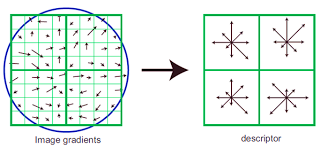
\includegraphics[width=0.4\textwidth]{Chapter4/Figs/gradients_and_binning.png}
  \textbf{
    \caption{ Image Gradients and Spatial/Orientation Binning.}
    \label{fig:6by6Grid}}
\end{figure}
%%%%%%%%%%%%%%%%%%%%%%%%%%%%%%%%%%%%%%%%%%%%%%%%%%%%%%%%%%%%%%%%%


Final step, is block normalising histograms within each block of cells. Because of gradient strengths varition as a result of local  illumination variations and foreground-background contrast, \citet{dalal2005histograms} found that some kind of illumination normalization must be done to be essential for good performance. They explored different normalization schemes to achieve that. Lets define first $v$ as the vector containing all the histograms for a given block, $\|v\|_k$ the k-norm of $v$ with $k\in 1,2$ and lets $\epsilon$  be a small constant. The normalization schemes are:

%%%%%%%%%%%%%%%%%%%%%%%%%%%%%%%%%%%%%%%%%%%%%%%%%%%%%%%%%%%%%%%%%
\begin{equation}\label{eq:L1-norm}
L1-norm: v\rightarrow \frac{v}{	\|v\|_2 + \epsilon}
\end{equation}
%%%%%%%%%%%%%%%%%%%%%%%%%%%%%%%%%%%%%%%%%%%%%%%%%%%%%%%%%%%%%%%%%

%%%%%%%%%%%%%%%%%%%%%%%%%%%%%%%%%%%%%%%%%%%%%%%%%%%%%%%%%%%%%%%%%
\begin{equation}\label{eq:L1-squared}
L1-squared norm: v\rightarrow \sqrt[]{\frac{v}{	\|v\|_2 + \epsilon}}
\end{equation}
%%%%%%%%%%%%%%%%%%%%%%%%%%%%%%%%%%%%%%%%%%%%%%%%%%%%%%%%%%%%%%%%%

%%%%%%%%%%%%%%%%%%%%%%%%%%%%%%%%%%%%%%%%%%%%%%%%%%%%%%%%%%%%%%%%%
\begin{equation}\label{eq:L2-norm}
L2-norm: v\rightarrow \frac{v}{\sqrt[]{	\|v\|_2^2 + \epsilon^2}}
\end{equation}
%%%%%%%%%%%%%%%%%%%%%%%%%%%%%%%%%%%%%%%%%%%%%%%%%%%%%%%%%%%%%%%%%

Dalal and Triggs experiments found that L1-norm-squared and L2-norm performs similar and achieves good results, but L1-norm decreases performance in a 5\%. Not normalizing reduce enormously the performance in around a 27\%. 


%%%%%%%%%%%%%%%%%%%%%%%%%%%%%%%%%%%%%%%%%%%%%%%%%%%%%%%%%%%%%%%%%
\begin{equation}\label{eq:NoOfLBPCells}
h_k
\end{equation}
%%%%%%%%%%%%%%%%%%%%%%%%%%%%%%%%%%%%%%%%%%%%%%%%%%%%%%%%%%%%%%%%%





\begin{figure}
\centering
\begin{subfigure}{.5\textwidth}
  \centering
  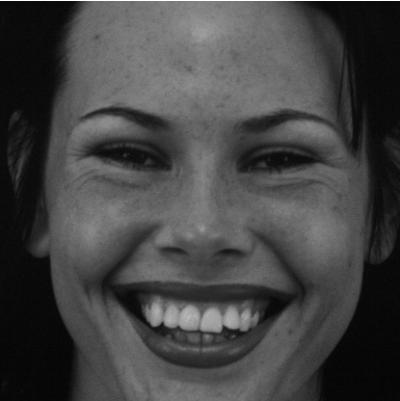
\includegraphics[width=.9\linewidth]{Chapter4/Figs/FaceHOG.png}
  \caption{A lady's face}
  \label{fig:sub1}
\end{subfigure}%
\begin{subfigure}{.5\textwidth}
  \centering
  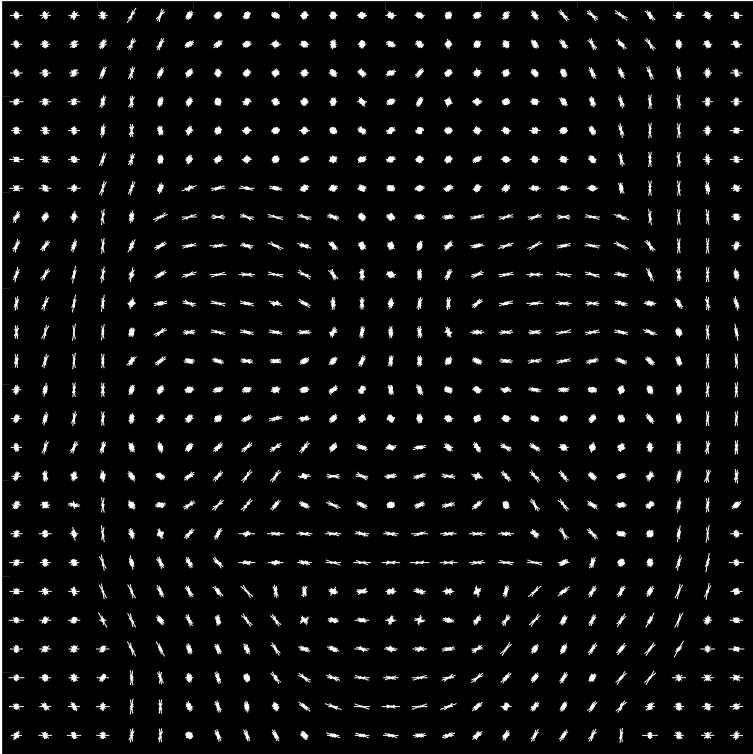
\includegraphics[width=.9\linewidth]{Chapter4/Figs/HOG.png}
  \caption{Visualization of extracted HOG }
  \label{fig:sub2}
\end{subfigure}
\caption{HOG descriptor Visualization}
\label{fig:test}
\end{figure}



HOG method has been wildly used in computer vision to recognise objects. HOG features have used in facial expression recognition with multi class RBF-SVM by extracting dense grid-based HOG features from images \citep{dahmane2011emotion}, where they used a cropped region from the aligned face and  divided into (48) squares 8 rows and 6 columns. In \citet{dahmane2011emotion}, GEMEP-FERA dataset has been used for training and testing 5 facial expressions anger, fear, joy, relief and sadness. As LBP, face have been divided into its main parts then extract each part's HOG features as shown in figure \ref{fig:HOGSyst}.


%%%%%%%%%%%%%%%%%%%%%%%%%%%%%%%%%%%%%%%%%%%%%%%%%%%%%%%%%%%%%%%%%
\begin{figure}[H]
\centering
  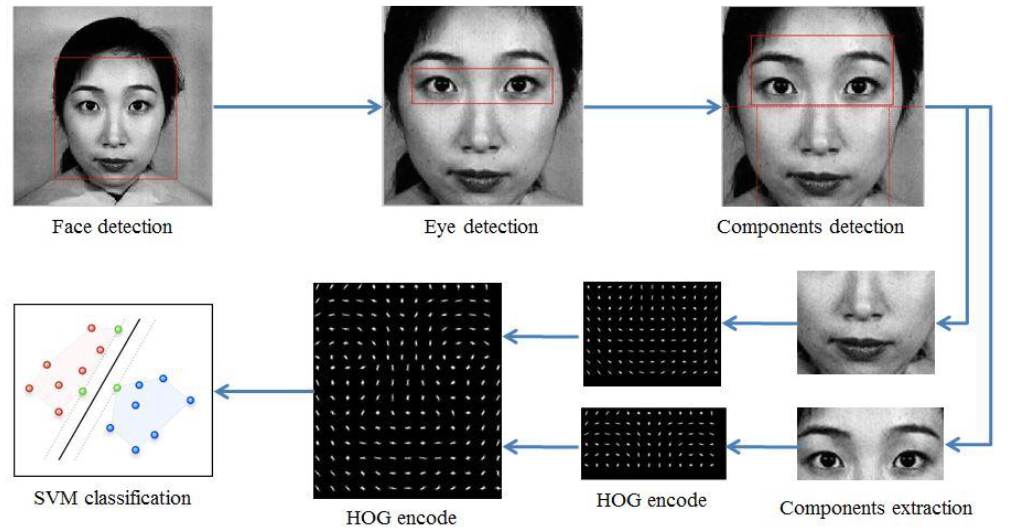
\includegraphics[width=0.65\textwidth]{Chapter2/Figs/HOGSyst.png}
  \textbf{
    \caption{An overview of the face recognition system with HOG \citep{chen2014facial}}
    \label{fig:HOGSyst}}
\end{figure}
%%%%%%%%%%%%%%%%%%%%%%%%%%%%%%%%%%%%%%%%%%%%%%%%%%%%%%%%%%%%%%%%%

HOG descriptor could be effectively exploited for facial expression recognition purposes has been carried out, and configuration of HOG parameters is able to give strong image descriptor which allows a high classification performance for facial expressions \citep{carcagni2015facial}.


%__________________________________________________________HOG__________________________________________________________________
%__________________________________________________________HOG__________________________________________________________________
%__________________________________________________________HOG__________________________________________________________________










\subsection{Scale-invariant feature transform (SIFT) and speeded up robust features (SURF)}

\textcolor{red}{
SIFT has been proposed by \citet{lowe2004distinctive} the image rotation, affine transformations, intensity, and viewpoint change in matching features. The SIFT algorithm has 4 basic steps. First is to estimate a scale space extremum using the Difference of Gaussian (DoG). Secondly, a key point localization where the key point candidates are localized and refined by eliminating the low contrast points. Thirdly, a key point orientation assignment based on local image gradient and lastly a descriptor generator to compute the local image descriptor for each key point based on image gradient magnitude and orientation \cite{karami2017image}.
}

The main SIFT advantage is its stability for images in different resolutions so it gives good performance in machine vision applications. In facial expression methods, SIFT features represent the same object with different expression and illumination\cite{zhang2008face}, figure \ref{fig:SIFT}  shows an example.
Researchers has used SIFT descriptor  with 2D and 3D images\citep{zhang2008face,berretti2010set,soyel2012localized}.   



%%%%%%%%%%%%%%%%%%%%%%%%%%%%%%%%%%%%%%%%%%%%%%%%%%%%%%%%%%%%%%%%%
\begin{figure}[H]
\centering
  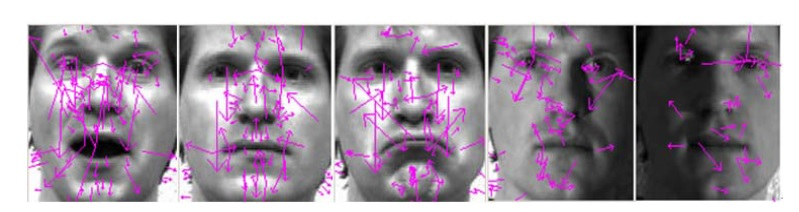
\includegraphics[width=0.8\textwidth]{Chapter2/Figs/SIFT.jpg}
  \textbf{
    \caption{Example of images with extracted SIFT features. The images represent the same object with different expression and illumination \citep{zhang2008face}}
    \label{fig:SIFT}}
\end{figure}
%%%%%%%%%%%%%%%%%%%%%%%%%%%%%%%%%%%%%%%%%%%%%%%%%%%%%%%%%%%%%%%%%


 Speeded Up Robust Features (SURF) were first presented by Herbert Bay as novel scale- and rotation-invariant interest point detectors and descriptors \citep{bay2006surf,bay2008speeded}. SURF is based on similar SIFT descriptor \citep{lowe1999object} properties.  SURF is faster than SIFT and gives as good a performance as SIFT \citep{panchal2013comparison}. (D-SURF) is a local feature detector and descriptor. It has been commonly used in computer vision tasks and object recognition classification. The D-SURF algorithm is based on the same principles and steps as SIFT; but the details in each step are different. The algorithm has three main parts: First "interest point detection" were selected at important locations in the image, for instant, and T-junctions, corners,blobs. To achieve that the algorithm uses very basic Hessian matrix approximation  because of its good performance in accuracy \citep{bay2008speeded}.The local next step is neighbourhood description and matching is smiler to the gradient information extracted by SIFT.
 
 



\newpage
\subsection{local Binary Pattern (LBP)}

Local binary patterns (LBP) were first proposed by \citet{ojala1996comparative} as a texture descriptor depending on statistical analysis, and since then it has been widely used for face analysis due to their classification performance \citep{zhou2013local}. The LPB operator compares each pixel in a 3x3 neighbourhood of the pixel to the central value and construct a binary digit number from the result, thus computing local texture characteristics. One of the most important advantages of LBP features is their tolerance against illumination variation\citep{shan2009facial}. Let us therefore define texture T in a local neighbourhood of a grayscale
image as the joint distribution of the gray levels of $P + 1 (P > 0)$ image
pixels:
%%%%%%%%%%%%%%%%%%%%%%%%%%%%%%%%%%%%%%%%%%%%%%%%%%%%%%%%%%%%%%%%%
\begin{equation}\label{eq:LBP_operator1}
T = t(g_c,g_0, ... , g_{P-1})
\end{equation}
%%%%%%%%%%%%%%%%%%%%%%%%%%%%%%%%%%%%%%%%%%%%%%%%%%%%%%%%%%%%%%%%%
where $g_c$ corresponds to the gray value of the centre pixel of a local neighbourhood. $g_p (p=0, ..., P-1)$ is the gray values of P equally spaced pixels on
a circle of radius $R (R > 0)$ that form a circularly symmetric set of neighbours.

%%%%%%%%%%%%%%%%%%%%%%%%%%%%%%%%%%%%%%%%%%%%%%%%%%%%%%%%%%%%%%%%%
 \begin{figure}[H]
\centering
  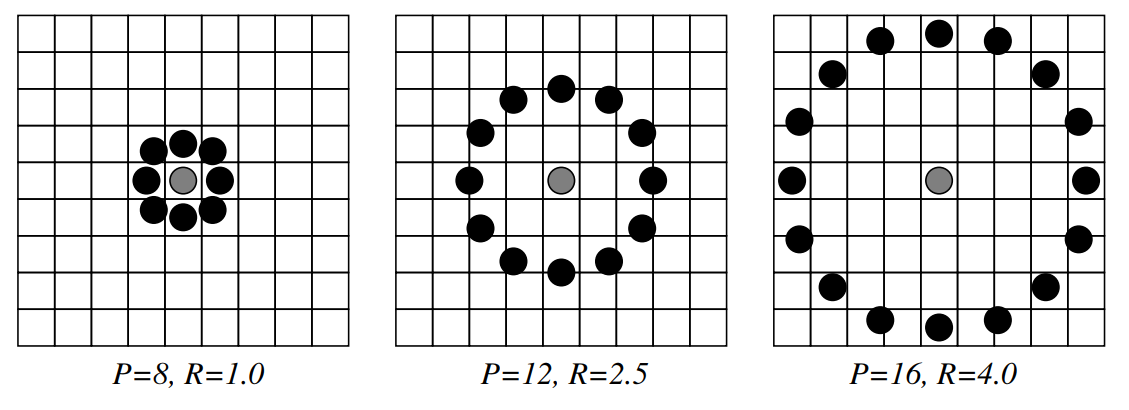
\includegraphics[width=90.5mm]{Chapter4/Figs/LBP.png}
  \textbf{\caption{Circularly symmetric neighbour sets. Samples that do not exactly
match the pixel grid are obtained via interpolation.}\label{fig:LBP_Circularly}}
    \end{figure}
%%%%%%%%%%%%%%%%%%%%%%%%%%%%%%%%%%%%%%%%%%%%%%%%%%%%%%%%%%%%%%%%%

Figure \ref{fig:LBP_Circularly} shows three examples of different values of P and R.  To achieve invariance with respect to any monotonic transformation of the
grayscale, only the signs of the differences are considered:

%%%%%%%%%%%%%%%%%%%%%%%%%%%%%%%%%%%%%%%%%%%%%%%%%%%%%%%%%%%%%%%%%
\begin{equation}\label{eq:e joint_difference_distribution}
T = t(s(g_0 - g_c) , ... , (g_{P-1} - g_c))
\end{equation}
%%%%%%%%%%%%%%%%%%%%%%%%%%%%%%%%%%%%%%%%%%%%%%%%%%%%%%%%%%%%%%%%%

where  corresponds to the grey value of the centre pixel $(x_c, y_c)$, in to the grey values of the 8 surrounding pixels, and function s(x) is defined as:

%%%%%%%%%%%%%%%%%%%%%%%%%%%%%%%%%%%%%%%%%%%%%%%%%%%%%%%%%%%%%%%%%
\begin{equation}\label{eq:LBP_operator2}
s(x) = \left\{ \begin{array}{rl}
 1 &\mbox{ if $x \geq	0$} \\
  0 &\mbox{ if $x < 0$}
       \end{array} \right.
  \end{equation}
%%%%%%%%%%%%%%%%%%%%%%%%%%%%%%%%%%%%%%%%%%%%%%%%%%%%%%%%%%%%%%%%%

The code characterizes thelocal image texture around (xc, yc):


%%%%%%%%%%%%%%%%%%%%%%%%%%%%%%%%%%%%%%%%%%%%%%%%%%%%%%%%%%%%%%%%%
\begin{equation}\label{eq:LBP_operator3}
LBP_{P,R}(x_c, y_c) =\sum_{p=0}^{P-1}  s(g_p  - g_c)2^n
\end{equation}
%%%%%%%%%%%%%%%%%%%%%%%%%%%%%%%%%%%%%%%%%%%%%%%%%%%%%%%%%%%%%%%%%


 
Number of neighbours used to compute the basic LBP for each pixel in the input image is 8 neighbours. Figure \ref{fig:LBPThresholdng} shows an example to LBP thresholding depending on 8 neighbours. LBP operator calculates the binary pattern according equation \ref{eq:LBP_operator2}. The final decimal number calculated by the weights for each neighbour.

In LBP,  image is divided into a number of cells which depends on the size if each cell. For example, if we have  image $I$ ,  and apply cell size $c$, the number of cells is calculated by the following  equation:

\textcolor{red}{
%%%%%%%%%%%%%%%%%%%%%%%%%%%%%%%%%%%%%%%%%%%%%%%%%%%%%%%%%%%%%%%%%
\begin{equation}\label{eq:NoOfLBPCells}
numCells = prod(floor(size(I)/CellSize))
  \end{equation}
%%%%%%%%%%%%%%%%%%%%%%%%%%%%%%%%%%%%%%%%%%%%%%%%%%%%%%%%%%%%%%%%%
}


%%%%%%%%%%%%%%%%%%%%%%%%%%%%%%%%%%%%%%%%%%%%%%%%%%%%%%%%%%%%%%%%%
\begin{figure}[H]
\centering
  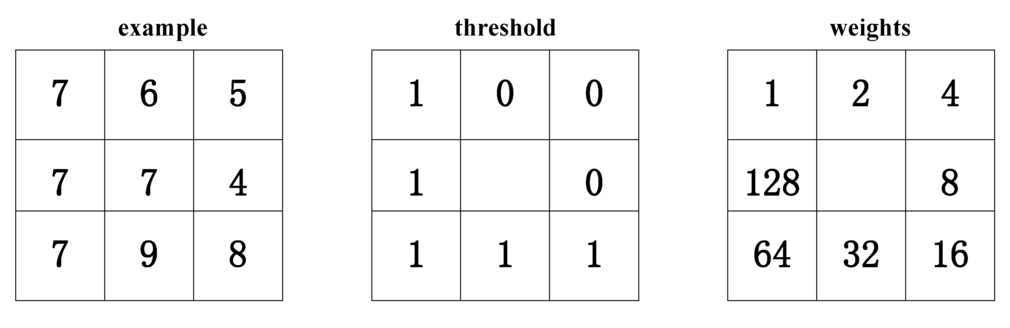
\includegraphics[width=0.42\textwidth]{Chapter4/Figs/LBPThresholdng_.png}
  \textbf{
    \caption{An example LBP thresholding depending on 8 neighbours. Pattern: 11110001, Decimal = 1+16+32+64+128=241.}
    \label{fig:LBPThresholdng}}
\end{figure}
%%%%%%%%%%%%%%%%%%%%%%%%%%%%%%%%%%%%%%%%%%%%%%%%%%%%%%%%%%%%%%%%%

%%%%%%%%%%%%%%%%%%%%%%%%%%%%%%%%%%%%%%%%%%%%%%%%%%%%%%%%%%%%%%%%%
\begin{figure}[H]
\centering
  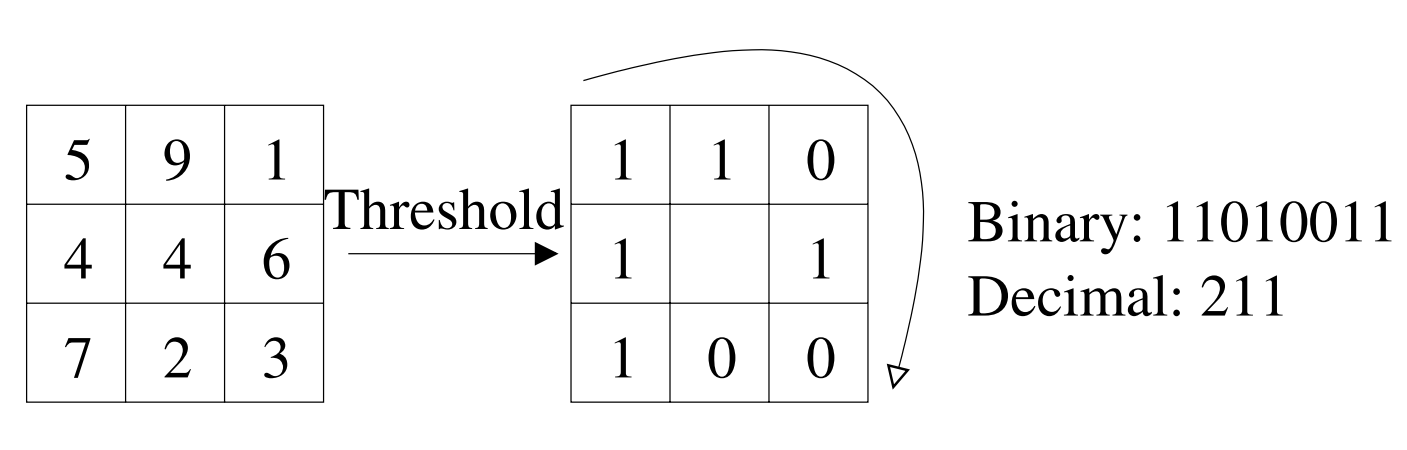
\includegraphics[width=0.7\textwidth]{Chapter2/Figs/LBPoperator.png}
  \textbf{
    \caption{The LBP operator\citep{ahonen2004face}}
    \label{fig:LBP_operator}}
\end{figure}
%%%%%%%%%%%%%%%%%%%%%%%%%%%%%%%%%%%%%%%%%%%%%%%%%%%%%%%%%%%%%%%%%


%%%%%%%%%%%%%%%%%%%%%%%%%%%%%%%%%%%%%%%%%%%%%%%%%%%%%%%%%%%%%%%%%
\begin{figure}[H]
\centering
  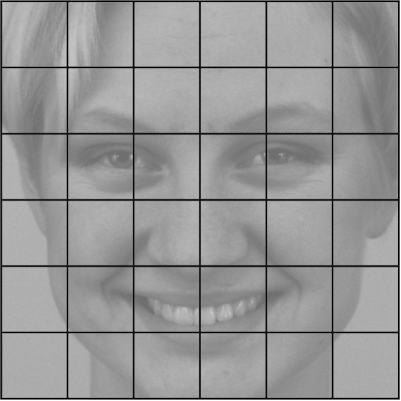
\includegraphics[width=0.25\textwidth]{Chapter4/Figs/6by6Grid.png}
  \textbf{
    \caption{An example 36 cells LBP}
    \label{fig:6by6Grid}}
\end{figure}
%%%%%%%%%%%%%%%%%%%%%%%%%%%%%%%%%%%%%%%%%%%%%%%%%%%%%%%%%%%%%%%%%



 

 LBP has been used with many classifiers to recognise facial expression because of its advantages, i.e., its tolerance of monotonic illumination changes and its computational simplicity \citep{huang2011local}. \citet{shan2005robust} used a simple Local Binary Patterns (LBP) with Support Vector Machine are (SVM). They have tested the extracted LBP features with linear, polynomial and RBF kernels SVM to classify seven facial expressions. They have used  Cohn Kanade Facial Expression Database which was produced by \citet{kanade2000comprehensive}, and contains faces of 100 university students in age from 18 to 30 years. \citet{shan2005robust} compared their results with Gabor wavelets, and they have found that LBP with SVM give better classification accuracy than Gabor wavelets, and save computational resource, and they proved that LBP gives good results with different resolutions even low-resolution images\citep{shan2005robust}. At the same area \cite{shan2009facial} have done a comprehensive study for facial expression recognition based on Local Binary Patterns and they found that LBP features are effective and efficient for facial expression recognition and it gives good results low-resolution images.
 
LBP have been used for frontal faces and for angle pose faces, \citep{moore2011local} have proposed a multi-view facial expression recognition using  some extensions including multi-scale local binary patterns ($LBP^{ms}$) and local gabor binary patterns ($LGBP$), and they have tested it on photos from multi-pie dataset \citep{gross2010multi} to see how see how head pose effects facial expression SVM classifier They have. 

During the last decade, researchers have prosed many methods to use LBP and LBP's extensions. Some of them have tried to divide face into equal blocks into grids \citep{moore2011local}, others have tried to divide face into its main parts eyes, nose and mouth like in \citet{khan2013framework} who have proposed pyramidal local binary pattern (PLBP) operator to recognise six facial expressions. The have tested the extracted features with four classifiers:2 nearest neighbour (2NN), Random forest (RF), SVM and C4.5 decision tree. They used in experiments two datasets: CK+ and FG-NET FEED.  





\section{Classification}
\subsection{Random Forest}

Random Forest (RF) is a popular method in computer vision because of its capacity to operate with  large multi-class datasets and give high accuracy results \citep{fanelli2011real} because of its great generalization ability, and it is very fast to train and parallelise \citep{breiman2001random,belle2008detection}. RF classifier contains a combination of tree classifiers, each one is created by a random vector independently from the input vector. Each tree gives a unit vote for the most popular class to classify an input vector \citep{breiman1999}.

To understand Random forest algorithm, we need to understand the basic idea of decision trees. Considering an input feature $X$ and an output $Y$ we need to learn a model can predict $Y$ for given feature $X$. Decision trees based on performing predictions using a sequence of simple decisions by ensemble of hierarchical binary decisions \citep{Random2012Medical}. In decision tree has top node called root connected with two children nodes, nodes at the bottom are called leaves as shown in figure \ref{fig:decisionTree}.    

%%%%%%%%%%%%%%%%%%%%%%%%%%%%%%%%%%%%%%%%%%%%%%%%%%%%%%%%%%%%%%%%%
\begin{figure}[H]
\centering
  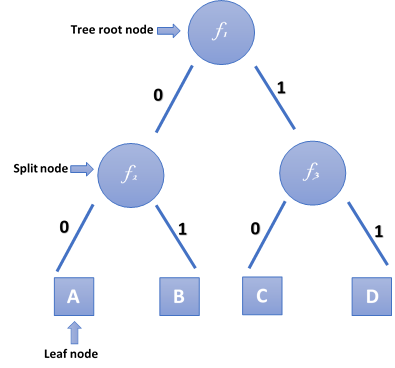
\includegraphics[width=0.4\textwidth]{Chapter2/Figs/decisionTree.png}
  \textbf{
    \caption{Simple decision tree}
    \label{fig:decisionTree}}
\end{figure}
%%%%%%%%%%%%%%%%%%%%%%%%%%%%%%%%%%%%%%%%%%%%%%%%%%%%%%%%%%%%%%%%%

The main idea of Random forest \citep{breiman2001random} $\mathcal{F}$ is to make a group (ensemble) of $T$ decision trees work together  $\mathcal{F} = \{ \mathbf{T_1}, ... ,\mathbf{T_t},...\mathbf{T_T} \}$ each tree node in random forests classifier is a weak classifier, each tree gets a "vote" in classifying \citep{breiman1996bagging,breiman1999,breiman2001random}. This combination of ensemble  decorrelated trees provides very good generalization. So, from the same dataset, many random samples can be generated to be processed by constructing decorrelated trees.  According to \citet{breiman2001random} randomization method "Bagging",  for given dataset $\mathbf{D} = \{ \mathbf{X}^{(n)}, Y^{(n)} \}_{n=1} ^ N$ is divided into random smaller dataset. Each data set $S_t$ called bootstrap. By growing a tree $\mathbf{T_t}$ for each bootstrap, an ensemble decision trees working together to make vote for a new unseen observation.  

%%%%%%%%%%%%%%%%%%%%%%%%%%%%%%%%%%%%%%%%%%%%%%%%%%%%%%%%%%%%%%%%%
\begin{figure}[H]
\centering
  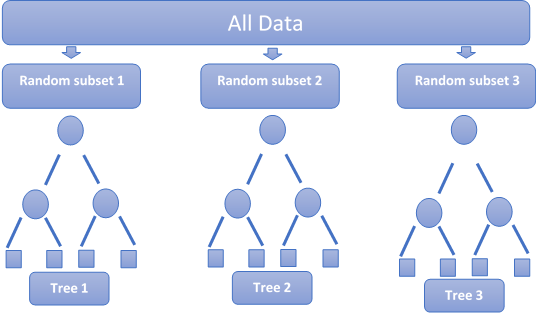
\includegraphics[width=0.70\textwidth]{Chapter2/Figs/RandomForest.png}
  \textbf{
    \caption{New subsets Randomisation by bagging method}
    \label{fig:RandomForest}}
\end{figure}
%%%%%%%%%%%%%%%%%%%%%%%%%%%%%%%%%%%%%%%%%%%%%%%%%%%%%%%%%%%%%%%%


In classification supervised training tasks, we have training data contains features and labels (output). Let given training dataset  $\{( \mathbf{X^{(n)}}, Y^{(n)}) \} _{n=1} ^N \in  \mathcal{X}  \times \mathcal{Y}$, where $\mathbf{X} \subset \mathcal{X}$ and $\mathbf{Y} \subset \mathcal{Y}$, for $\mathcal{X} \subset  \mathbb{R}^D$ the features space and the output space  $\mathcal{Y} \subset  \mathbb{R}$, which is a finite set of $K$ discrete values $\mathcal{Y} = \{y_1,...,y_k,...,y_K\}$  represent the the classes . Let us consider the partition $\mathcal{P}_t =\{ \mathcal{C}_t^{(zt)} \}  _{z_t=1} ^{Z_t}$ built by the random tree  $\mathbf{T}_t$ \citep{Random2012Medical}. Class posteriors can be simply approximated in each cell $\mathcal{C} ^{(zt)}$ of $\mathcal{P}_t$ as follows:

%%%%%%%%%%%%%%%%%%%%%%%%%%%%%%%%%%%%%%%%%%%%%%%%%%%%%%%%%%%%%%%%%
\begin{equation}\label{eq:cell_posteriori}
P(y_k \mid \mathbf{X} \in \mathcal{C}_t ^ {(z_t)} ,  \mathcal{P}_t) = \frac{\mid \{ \mathbf{X}^{(n)} \in \mathcal{C}_t ^ (z_t), Y^{(n)} = y_k \} \mid } {\mid \{  \mathbf{X}^{(n)} \in \mathcal{C}_t ^ {(z_t)} \} \mid }
\end{equation}
%%%%%%%%%%%%%%%%%%%%%%%%%%%%%%%%%%%%%%%%%%%%%%%%%%%%%%%%%%%%%%%%




In classification tasks, if a trained model is given a new unseen feature and it should  predict to which class does it  refer by sending the unseen feature through all trees of the forest and combining tree posteriors.   class prediction for a new observation is the class that yields the largest weighted average of the class posterior probabilities computed using selected trees only.  For each class $c \in \mathcal{C}$ and each tree $t=1, ... ,T$. Prediction for new observation $x$ computes $\hat{P}(c\mid x)$ to estimate posterior probability of class $c$ using $t$. $\mathcal{C}$ is the set of all distinct classes in the training data:

%%%%%%%%%%%%%%%%%%%%%%%%%%%%%%%%%%%%%%%%%%%%%%%%%%%%%%%%%%%%%%%%%
\begin{equation}\label{eq:maximum_posteriori}
\hat{P}_{bag}= \frac{1}{\sum_{t=1}^{T} \alpha_t I(t\in S)} \sum_{t=1}^{T} \alpha_t \hat{y_t} I(t\in S)
\end{equation}
%%%%%%%%%%%%%%%%%%%%%%%%%%%%%%%%%%%%%%%%%%%%%%%%%%%%%%%%%%%%%%%%
where $\hat{y_t}$ is the prediction from tree t in the ensemble, $S$ is the set of indices of selected trees that comprise the prediction and $\alpha_t$ is the weight of tree.


%%%%%%%%%%%%%%%%%%%%%%%%%%%%%%%%%%%%%%%%%%%%%%%%%%%%%%%%%%%%%%%%%
\begin{equation}\label{eq:maximum_posteriori}
\hat{Y}_{bag}= argmax_{c \in \mathcal{C}} \{ P_{bag}(c \mid x)\}
\end{equation}.
%%%%%%%%%%%%%%%%%%%%%%%%%%%%%%%%%%%%%%%%%%%%%%%%%%%%%%%%%%%%%%%%



 


The RFs classifier has proficient power to gauge the importance of each features variable (predictor) \citep{breiman2001random} by calculating how much a prediction error increases or decrease  when (OOB) data for that variable is permuted while all others are passed on unaltered. The calculations are carried out tree by tree as the random forest is constructed \citep{breiman2001random,breiman2002manual,liaw2002classification}.


Breiman has proposed a method to evaluate the variable importance by measuring the Mean Decrease Accuracy of the forest when the values of $X_m$ are randomly permuted in the out-of-bag samples. Suppose we have M input variables. After each tree is built, the values of the $m_{th}$ variable in the out-of-bag examples are randomly permuted and the out-of-bag data is run down the corresponding tree. The classification given for each $x_n$ that is out of bag is saved. This is repeated for $m=1,2, ... , M$. At the end of the run, the plurality of out-of-bag class votes for $x_n$ with the $m_th$ variable noised up is compared with the true class label of $x_n$ to give a misclassification rate. The output is the percent increase in misclassification rate as compared to the out-of-bag rate (with all variables intact).\citep{breiman2001random,louppe2013understanding}.


\subsection{Out-of-bag (OOB) error }
In classification problems, (OOB) error returns the weighted misclassification rate.

oobError predicts classes for all out-of-bag observations.

The weighted misclassification rate estimate depends on the value of 'Mode'.
If you specify 'Mode','Individual', then oobError sets any in bag observations within a selected tree to the predicted, weighted, most popular class over all training responses. If there are multiple most popular classes, error considers the one listed first in the Class Names property of the TreeBagger model the most popular. Then, oobError computes the weighted misclassification rate for each selected tree.

If you specify 'Mode','Cumulative', then ooError returns a vector of cumulative, weighted misclassification rates, where et* is the cumulative, weighted misclassification rate for selected tree t. To compute et*, for each observation that is out of bag for at least one tree through tree t, oobError finds the predicted, cumulative, weighted most popular class through tree t. oobError sets observations that are in bag for all selected trees through tree t to the weighted, most popular class over all training responses. If there are multiple most popular classes, error considers the one listed first in the ClassNames property of the TreeBagger model the most popular. Then, oobError computes et*.


If you specify 'Mode','Ensemble', then, for each observation that is out of bag for at least one tree, oobError computes the weighted, most popular class over all selected trees. oobError sets observations that are in bag for all selected trees through tree t to the predicted, weighted, most popular class over all training responses. If there are multiple most popular classes, error considers the one listed first in the Class Names property of the TreeBagger model the most popular. Then, oobError computes the weighted misclassification rate , which is the same as the final, cumulative, weighted misclassification rate.


\subsection{Support vector machine}
SVM was first introduced by Vladimir Vapnik in 1979 and first published in 1995.









\section{Conclusion}
